\documentclass[t]{beamer}
\definecolor{rrblitbackground}{rgb}{0.55, 0.3, 0.1}

\newenvironment{rtbliteral}{

\begin{ttfamily}

\color{rrblitbackground}

}{

\end{ttfamily}

}

\usepackage{fancyvrb}

\usepackage{color}

\usetheme{metropolis}

\setbeameroption{hide notes}


\makeatletter
\def\PY@reset{\let\PY@it=\relax \let\PY@bf=\relax%
    \let\PY@ul=\relax \let\PY@tc=\relax%
    \let\PY@bc=\relax \let\PY@ff=\relax}
\def\PY@tok#1{\csname PY@tok@#1\endcsname}
\def\PY@toks#1+{\ifx\relax#1\empty\else%
    \PY@tok{#1}\expandafter\PY@toks\fi}
\def\PY@do#1{\PY@bc{\PY@tc{\PY@ul{%
    \PY@it{\PY@bf{\PY@ff{#1}}}}}}}
\def\PY#1#2{\PY@reset\PY@toks#1+\relax+\PY@do{#2}}

\expandafter\def\csname PY@tok@s2\endcsname{\def\PY@tc##1{\textcolor[rgb]{0.73,0.13,0.13}{##1}}}
\expandafter\def\csname PY@tok@se\endcsname{\let\PY@bf=\textbf\def\PY@tc##1{\textcolor[rgb]{0.73,0.40,0.13}{##1}}}
\expandafter\def\csname PY@tok@vg\endcsname{\def\PY@tc##1{\textcolor[rgb]{0.10,0.09,0.49}{##1}}}
\expandafter\def\csname PY@tok@kr\endcsname{\let\PY@bf=\textbf\def\PY@tc##1{\textcolor[rgb]{0.00,0.50,0.00}{##1}}}
\expandafter\def\csname PY@tok@mo\endcsname{\def\PY@tc##1{\textcolor[rgb]{0.40,0.40,0.40}{##1}}}
\expandafter\def\csname PY@tok@mb\endcsname{\def\PY@tc##1{\textcolor[rgb]{0.40,0.40,0.40}{##1}}}
\expandafter\def\csname PY@tok@sd\endcsname{\let\PY@it=\textit\def\PY@tc##1{\textcolor[rgb]{0.73,0.13,0.13}{##1}}}
\expandafter\def\csname PY@tok@sc\endcsname{\def\PY@tc##1{\textcolor[rgb]{0.73,0.13,0.13}{##1}}}
\expandafter\def\csname PY@tok@bp\endcsname{\def\PY@tc##1{\textcolor[rgb]{0.00,0.50,0.00}{##1}}}
\expandafter\def\csname PY@tok@ch\endcsname{\let\PY@it=\textit\def\PY@tc##1{\textcolor[rgb]{0.25,0.50,0.50}{##1}}}
\expandafter\def\csname PY@tok@kc\endcsname{\let\PY@bf=\textbf\def\PY@tc##1{\textcolor[rgb]{0.00,0.50,0.00}{##1}}}
\expandafter\def\csname PY@tok@nd\endcsname{\def\PY@tc##1{\textcolor[rgb]{0.67,0.13,1.00}{##1}}}
\expandafter\def\csname PY@tok@il\endcsname{\def\PY@tc##1{\textcolor[rgb]{0.40,0.40,0.40}{##1}}}
\expandafter\def\csname PY@tok@ni\endcsname{\let\PY@bf=\textbf\def\PY@tc##1{\textcolor[rgb]{0.60,0.60,0.60}{##1}}}
\expandafter\def\csname PY@tok@ne\endcsname{\let\PY@bf=\textbf\def\PY@tc##1{\textcolor[rgb]{0.82,0.25,0.23}{##1}}}
\expandafter\def\csname PY@tok@gt\endcsname{\def\PY@tc##1{\textcolor[rgb]{0.00,0.27,0.87}{##1}}}
\expandafter\def\csname PY@tok@vc\endcsname{\def\PY@tc##1{\textcolor[rgb]{0.10,0.09,0.49}{##1}}}
\expandafter\def\csname PY@tok@s\endcsname{\def\PY@tc##1{\textcolor[rgb]{0.73,0.13,0.13}{##1}}}
\expandafter\def\csname PY@tok@nc\endcsname{\let\PY@bf=\textbf\def\PY@tc##1{\textcolor[rgb]{0.00,0.00,1.00}{##1}}}
\expandafter\def\csname PY@tok@mh\endcsname{\def\PY@tc##1{\textcolor[rgb]{0.40,0.40,0.40}{##1}}}
\expandafter\def\csname PY@tok@c1\endcsname{\let\PY@it=\textit\def\PY@tc##1{\textcolor[rgb]{0.25,0.50,0.50}{##1}}}
\expandafter\def\csname PY@tok@c\endcsname{\let\PY@it=\textit\def\PY@tc##1{\textcolor[rgb]{0.25,0.50,0.50}{##1}}}
\expandafter\def\csname PY@tok@gd\endcsname{\def\PY@tc##1{\textcolor[rgb]{0.63,0.00,0.00}{##1}}}
\expandafter\def\csname PY@tok@gr\endcsname{\def\PY@tc##1{\textcolor[rgb]{1.00,0.00,0.00}{##1}}}
\expandafter\def\csname PY@tok@k\endcsname{\let\PY@bf=\textbf\def\PY@tc##1{\textcolor[rgb]{0.00,0.50,0.00}{##1}}}
\expandafter\def\csname PY@tok@gh\endcsname{\let\PY@bf=\textbf\def\PY@tc##1{\textcolor[rgb]{0.00,0.00,0.50}{##1}}}
\expandafter\def\csname PY@tok@sh\endcsname{\def\PY@tc##1{\textcolor[rgb]{0.73,0.13,0.13}{##1}}}
\expandafter\def\csname PY@tok@gu\endcsname{\let\PY@bf=\textbf\def\PY@tc##1{\textcolor[rgb]{0.50,0.00,0.50}{##1}}}
\expandafter\def\csname PY@tok@mi\endcsname{\def\PY@tc##1{\textcolor[rgb]{0.40,0.40,0.40}{##1}}}
\expandafter\def\csname PY@tok@m\endcsname{\def\PY@tc##1{\textcolor[rgb]{0.40,0.40,0.40}{##1}}}
\expandafter\def\csname PY@tok@sx\endcsname{\def\PY@tc##1{\textcolor[rgb]{0.00,0.50,0.00}{##1}}}
\expandafter\def\csname PY@tok@kn\endcsname{\let\PY@bf=\textbf\def\PY@tc##1{\textcolor[rgb]{0.00,0.50,0.00}{##1}}}
\expandafter\def\csname PY@tok@vi\endcsname{\def\PY@tc##1{\textcolor[rgb]{0.10,0.09,0.49}{##1}}}
\expandafter\def\csname PY@tok@gi\endcsname{\def\PY@tc##1{\textcolor[rgb]{0.00,0.63,0.00}{##1}}}
\expandafter\def\csname PY@tok@s1\endcsname{\def\PY@tc##1{\textcolor[rgb]{0.73,0.13,0.13}{##1}}}
\expandafter\def\csname PY@tok@cpf\endcsname{\let\PY@it=\textit\def\PY@tc##1{\textcolor[rgb]{0.25,0.50,0.50}{##1}}}
\expandafter\def\csname PY@tok@cm\endcsname{\let\PY@it=\textit\def\PY@tc##1{\textcolor[rgb]{0.25,0.50,0.50}{##1}}}
\expandafter\def\csname PY@tok@nf\endcsname{\def\PY@tc##1{\textcolor[rgb]{0.00,0.00,1.00}{##1}}}
\expandafter\def\csname PY@tok@gs\endcsname{\let\PY@bf=\textbf}
\expandafter\def\csname PY@tok@no\endcsname{\def\PY@tc##1{\textcolor[rgb]{0.53,0.00,0.00}{##1}}}
\expandafter\def\csname PY@tok@sr\endcsname{\def\PY@tc##1{\textcolor[rgb]{0.73,0.40,0.53}{##1}}}
\expandafter\def\csname PY@tok@ge\endcsname{\let\PY@it=\textit}
\expandafter\def\csname PY@tok@vm\endcsname{\def\PY@tc##1{\textcolor[rgb]{0.10,0.09,0.49}{##1}}}
\expandafter\def\csname PY@tok@nn\endcsname{\let\PY@bf=\textbf\def\PY@tc##1{\textcolor[rgb]{0.00,0.00,1.00}{##1}}}
\expandafter\def\csname PY@tok@kt\endcsname{\def\PY@tc##1{\textcolor[rgb]{0.69,0.00,0.25}{##1}}}
\expandafter\def\csname PY@tok@dl\endcsname{\def\PY@tc##1{\textcolor[rgb]{0.73,0.13,0.13}{##1}}}
\expandafter\def\csname PY@tok@na\endcsname{\def\PY@tc##1{\textcolor[rgb]{0.49,0.56,0.16}{##1}}}
\expandafter\def\csname PY@tok@gp\endcsname{\let\PY@bf=\textbf\def\PY@tc##1{\textcolor[rgb]{0.00,0.00,0.50}{##1}}}
\expandafter\def\csname PY@tok@err\endcsname{\def\PY@bc##1{\setlength{\fboxsep}{0pt}\fcolorbox[rgb]{1.00,0.00,0.00}{1,1,1}{\strut ##1}}}
\expandafter\def\csname PY@tok@nt\endcsname{\let\PY@bf=\textbf\def\PY@tc##1{\textcolor[rgb]{0.00,0.50,0.00}{##1}}}
\expandafter\def\csname PY@tok@o\endcsname{\def\PY@tc##1{\textcolor[rgb]{0.40,0.40,0.40}{##1}}}
\expandafter\def\csname PY@tok@sb\endcsname{\def\PY@tc##1{\textcolor[rgb]{0.73,0.13,0.13}{##1}}}
\expandafter\def\csname PY@tok@ss\endcsname{\def\PY@tc##1{\textcolor[rgb]{0.10,0.09,0.49}{##1}}}
\expandafter\def\csname PY@tok@sa\endcsname{\def\PY@tc##1{\textcolor[rgb]{0.73,0.13,0.13}{##1}}}
\expandafter\def\csname PY@tok@nv\endcsname{\def\PY@tc##1{\textcolor[rgb]{0.10,0.09,0.49}{##1}}}
\expandafter\def\csname PY@tok@w\endcsname{\def\PY@tc##1{\textcolor[rgb]{0.73,0.73,0.73}{##1}}}
\expandafter\def\csname PY@tok@kd\endcsname{\let\PY@bf=\textbf\def\PY@tc##1{\textcolor[rgb]{0.00,0.50,0.00}{##1}}}
\expandafter\def\csname PY@tok@cs\endcsname{\let\PY@it=\textit\def\PY@tc##1{\textcolor[rgb]{0.25,0.50,0.50}{##1}}}
\expandafter\def\csname PY@tok@mf\endcsname{\def\PY@tc##1{\textcolor[rgb]{0.40,0.40,0.40}{##1}}}
\expandafter\def\csname PY@tok@si\endcsname{\let\PY@bf=\textbf\def\PY@tc##1{\textcolor[rgb]{0.73,0.40,0.53}{##1}}}
\expandafter\def\csname PY@tok@nl\endcsname{\def\PY@tc##1{\textcolor[rgb]{0.63,0.63,0.00}{##1}}}
\expandafter\def\csname PY@tok@go\endcsname{\def\PY@tc##1{\textcolor[rgb]{0.53,0.53,0.53}{##1}}}
\expandafter\def\csname PY@tok@ow\endcsname{\let\PY@bf=\textbf\def\PY@tc##1{\textcolor[rgb]{0.67,0.13,1.00}{##1}}}
\expandafter\def\csname PY@tok@nb\endcsname{\def\PY@tc##1{\textcolor[rgb]{0.00,0.50,0.00}{##1}}}
\expandafter\def\csname PY@tok@kp\endcsname{\def\PY@tc##1{\textcolor[rgb]{0.00,0.50,0.00}{##1}}}
\expandafter\def\csname PY@tok@fm\endcsname{\def\PY@tc##1{\textcolor[rgb]{0.00,0.00,1.00}{##1}}}
\expandafter\def\csname PY@tok@cp\endcsname{\def\PY@tc##1{\textcolor[rgb]{0.74,0.48,0.00}{##1}}}

\def\PYZbs{\char`\\}
\def\PYZus{\char`\_}
\def\PYZob{\char`\{}
\def\PYZcb{\char`\}}
\def\PYZca{\char`\^}
\def\PYZam{\char`\&}
\def\PYZlt{\char`\<}
\def\PYZgt{\char`\>}
\def\PYZsh{\char`\#}
\def\PYZpc{\char`\%}
\def\PYZdl{\char`\$}
\def\PYZhy{\char`\-}
\def\PYZsq{\char`\'}
\def\PYZdq{\char`\"}
\def\PYZti{\char`\~}
% for compatibility with earlier versions
\def\PYZat{@}
\def\PYZlb{[}
\def\PYZrb{]}
\makeatother

% generated by Docutils <http://docutils.sourceforge.net/>
\usepackage{cmap} % fix search and cut-and-paste in Acrobat
\usepackage{ifthen}
\usepackage[T1]{fontenc}
\usepackage[utf8]{inputenc}
\usepackage{amsmath}
\usepackage{graphicx}
\setcounter{secnumdepth}{0}

%%% Custom LaTeX preamble
% PDF Standard Fonts
\usepackage{mathptmx} % Times
\usepackage[scaled=.90]{helvet}
\usepackage{courier}

%%% User specified packages and stylesheets
\usepackage{my_beamer}

%%% Fallback definitions for Docutils-specific commands

% admonition (specially marked topic)
\providecommand{\DUadmonition}[2][class-arg]{%
  % try \DUadmonition#1{#2}:
  \ifcsname DUadmonition#1\endcsname%
    \csname DUadmonition#1\endcsname{#2}%
  \else
    \begin{center}
      \fbox{\parbox{0.9\linewidth}{#2}}
    \end{center}
  \fi
}

% inline markup (custom roles)
% \DUrole{#1}{#2} tries \DUrole#1{#2}
\providecommand*{\DUrole}[2]{%
  % backwards compatibility: try \docutilsrole#1{#2}
  \ifcsname docutilsrole#1\endcsname%
    \csname docutilsrole#1\endcsname{#2}%
  \else
    \csname DUrole#1\endcsname{#2}%
  \fi%
}

% hyperlinks:
\ifthenelse{\isundefined{\hypersetup}}{
  \usepackage[colorlinks=true,linkcolor=blue,urlcolor=blue]{hyperref}
  \usepackage{bookmark}
  \urlstyle{same} % normal text font (alternatives: tt, rm, sf)
}{}
\hypersetup{
  pdftitle={Alternating Finite Automata for Deciding Presburger Arithmetic},
  pdfauthor={Kei Shirakizawa (JAIST)}
}


%%% Body
\begin{document}

% Document title
\title[Alternating Finite Automata for Deciding Presburger Arithmetic]{Alternating Finite Automata for Deciding Presburger Arithmetic%
  \label{alternating-finite-automata-for-deciding-presburger-arithmetic}}
\author[Kei Shirakizawa (JAIST)]{Kei Shirakizawa (JAIST)}
\date{}
\maketitle


\section{Introduction%
  \label{introduction}%
}

\begin{frame}[fragile]
\frametitle{Automata-based Decision Procedure for Presburger Arithmetic}


\DUrole{raw}{\todo{State problem specification and introduce automata-based
decision procedure.}}

\begin{description}
\item[{Problem}] \leavevmode 
On input a Presburger Arithmetic formula, check SAT/validity.

\item[{Procedure}] \leavevmode 
(Boudet, Comon)
\begin{enumerate}

\item Regular set as solution space

\item Check language emptiness
\end{enumerate}

\end{description}

\end{frame}

\begin{frame}[fragile]
\frametitle{Optimized Methods for Automata-based Decision Procedure}


\DUrole{raw}{\todo{Introduce Antichain and Bisimulation}}
\begin{block}{Background}

TODO
\end{block}
\begin{block}{Antichain algorithm}

TODO
\end{block}
\begin{block}{Bisimulation up to congruence}

TODO
\end{block}

\end{frame}

\begin{frame}[fragile]
\frametitle{Topics}


\begin{description}
\item[{Problem}] \leavevmode 
SAT/validity checking of Presburger Arithmetic

\item[{Procedure}] \leavevmode 
Automata construction followed by emptiness checking

\item[{Limitation}] \leavevmode 
EXPTIME-COMPLETE

\item[{Aim}] \leavevmode 
Optimize the decision procedure

\end{description}
\begin{block}{Optimization techniques}
\begin{itemize}

\item \textbf{Antichain Algorithm}: Language universality

\item \textbf{Bisimulation up to Congruence}: Language equality
\end{itemize}
\end{block}
\begin{block}{Contribution}
\begin{itemize}

\item Alternating Finite Automaton(AFA)

\item SAT encoding
\end{itemize}
\end{block}

\end{frame}

\begin{frame}[fragile]
\frametitle{Related Works}


\DUrole{raw}{\todo{Collect works on automatic structure, optimization,
decision procedures}}
\begin{block}{So-called Automatic Structure}

WS1S is a logic with a model
\end{block}
\begin{block}{Optimization Techniques}

Nested Antichain for WS1S
\end{block}
\begin{block}{Decision Procedures}

Coalgebraic approach
\end{block}

\end{frame}


\section{Preliminaries%
  \label{preliminaries}%
}

\begin{frame}[fragile]
\frametitle{Presburger Arithmetic}


\DUrole{raw}{\todo{Define PA}}
$\forall x \ldotp$ and $\exists y \ldotp$.

\begin{example}[Presburger Arithmetic]
     \todo{Show example}
\end{example}

\end{frame}

\begin{frame}[fragile]
\frametitle{Finite Automata}


\DUrole{raw}{\todo{Define FA}}

\begin{definition}[NFA]
    \todo{Define NFA}
\end{definition}

\begin{example}[NFA]
    \todo{Show example}
\end{example}

\end{frame}

\begin{frame}[fragile]
\frametitle{Automata-based Decision Procedure for Presburger Arithmetic}


\DUrole{raw}{\todo{Explain/demonstrate Boudet Comon}}
\begin{block}{Boudet Common}

Automata onstruction
\end{block}

\end{frame}

\begin{frame}[fragile]
\frametitle{Projection for Existential Quantifier}


\DUrole{raw}{\todo{Explain/demonstrate homomorphism and projection}}

\begin{theorem}[Closed under homomorphism]
  A regular language is closed under homomorphism.
\end{theorem}

\end{frame}


\section{Optimization Techniques%
  \label{optimization-techniques}%
}

\begin{frame}[fragile]
\frametitle{Antichain Algorithm}


\( \subseteq \)

\noindent\makebox[\linewidth][c]{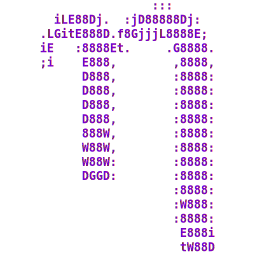
\includegraphics[height=0.75\textheight]{images/nano.pdf}}

\end{frame}

\begin{frame}[fragile]
\frametitle{Bisimulation up to Congruence}


\( \cong \)

\noindent\makebox[\linewidth][c]{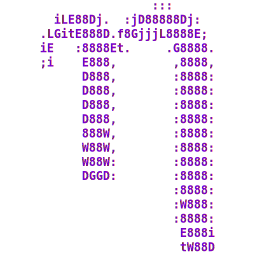
\includegraphics[height=0.75\textheight]{images/nano.pdf}}

\end{frame}


\section{AFA-based Decision Procedure%
  \label{afa-based-decision-procedure}%
}

\begin{frame}[fragile]
\frametitle{Alternating Finite Automaton}


\DUrole{raw}{todo{Define AFA and explain/demonstrate NFA equivalence.}}

\end{frame}

\begin{frame}[fragile]
\frametitle{NFA to AFA Translation}


\DUrole{raw}{todo{Explain/demonstrate AFA translation.}}

\end{frame}

\begin{frame}[fragile]
\frametitle{AC in AFA}


\DUrole{raw}{\todo{Explain/demonstrate AC in AFA setting}}

\(
    \alpha \equiv q_0[\delta(q_0, a)/q_0, \ldots \delta(q_n, a)/q_n]
\)
\( \alpha \Rightarrow \beta \)

\end{frame}

\begin{frame}[fragile]
\frametitle{BC in AFA}


\DUrole{raw}{\todo{Explain/demonstrate BC in AFA setting}}

\(
    \alpha \equiv q_0[\delta(q_0, a)/q_0, \ldots \delta(q_n, a)/q_n]
\)
\( \alpha \vee \gamma \Rightarrow \beta \)

\end{frame}

\begin{frame}[fragile]
\frametitle{AFA-based Optimization Method}


\DUrole{raw}{\todo{Define the procedure}}

\end{frame}

\begin{frame}[fragile]
\frametitle{Example (AFA-based Optimization Method)}


\DUrole{raw}{\todo{Exemplify AFA-based Optimization Method}}

\end{frame}

\begin{frame}[fragile]
\frametitle{SAT Encoding}


\DUrole{raw}{\todo{Explain/demonstrate SAT encoding}}

\end{frame}

\begin{frame}[fragile]
\frametitle{Example (SAT Encoding)}


\DUrole{raw}{\todo{Exemplify SAT encoding}}

\end{frame}


\section{Conclusion%
  \label{conclusion}%
}

\begin{frame}[fragile]
\frametitle{Evaluation}


\DUrole{raw}{\todo{Evaluate experimental result}}

Nothing to evaluate.

\end{frame}

\begin{frame}[fragile]
\frametitle{Conclusion}


\DUrole{raw}{\todo{Conclude contribution of this work}}

\begin{description}
\item[{Problem}] \leavevmode 
Check $\varphi \models \mathit{PA}$

\item[{Procedure}] \leavevmode \begin{enumerate}

\item DFA -> AFA

\item Enumerate AFA's reachable state minimizing it

\item Ordering -> CNF and feed it to SAT solver
\end{enumerate}

\end{description}
\begin{block}{Comparison of techniques}
\begin{itemize}

\item Antichain Algorithm: Check $\mathcal{L}(\mathcal{A}) = \Sigma^*$

\item Bisimulation up to Congruence: $\mathcal{L}(\mathcal{A}) = \mathcal{L}(\mathcal{B})$

\item \textbf{AFA-based technique}: $\mathcal{L}(\mathcal{A}) = \varnothing$
\end{itemize}
\end{block}

\end{frame}

\begin{frame}[fragile]
\frametitle{Future work}


\DUrole{raw}{\todo{Enumerate further direction of this work}}
\begin{block}{So-called Automatic Structure}

WS1S is a logic with a model
\end{block}
\begin{block}{Optimization Techniques}

Nested Antichain for WS1S
\end{block}
\begin{block}{Decision Procedures}

Coalgebraic approach
\end{block}

\end{frame}

\end{document}
